\documentclass[10pt,letterpaper,twoside]{article}
\usepackage{code/manuscript_assets/researchpreprint}
\usepackage[T1]{fontenc}
\usepackage{amsmath,amssymb,amsfonts,mathtools,amsthm,bm}
\usepackage{booktabs,tabularx,array}
\usepackage{graphicx}
\usepackage{xcolor}
\usepackage{microtype}
\usepackage{hyperref}
\usepackage{url}
\hypersetup{hidelinks}
\setlength{\emergencystretch}{3em}
\newtheorem{theorem}{Theorem}
\newtheorem{proposition}{Proposition}
\newtheorem{corollary}{Corollary}
\newcommand{\R}{\mathbb{R}}
\newcommand{\norm}[1]{\left\lVert #1\right\rVert}
\newcommand{\trans}{\mathsf T}
\newcommand{\method}{\textsc{CF-MFRP}}
\newcommand{\PrimaryBaseMSE}{0.416046}
\newcommand{\PrimaryMethodMSE}{0.398645}
\newcommand{\ExternalBaseMSE}{0.418608}
\newcommand{\ExternalMethodMSE}{0.412775}
\newcommand{\PrimaryRelativeGain}{4.18\%}
\newcommand{\ExternalRelativeGain}{1.39\%}
\newcommand{\SelectedLambda}{10}
\newcommand{\SelectedBlend}{1.000}
\newcommand{\PrimaryResidual}{9.63e-10}
\newcommand{\ExternalResidual}{9.60e-10}
\newcommand{\PrimaryStorage}{1.148\%}
\newcommand{\ExternalStorage}{0.714\%}
\newcommand{\BatchSpeedRatio}{1.21}
\newcommand{\BatchAgreement}{2.66e-16}
\newcommand{\RepeatWins}{5}


\begin{document}

\title{Leakage-Audited Matrix-Free Residual Propagation for Gene Measurements}
\author{Molena Huynh}
\email{molena.huynh@jmp.com}
\affiliation{North Carolina State University}
\date{July 31, 2026}

\maketitle

\begin{abstract}
We revisit held-out marker-gene prediction on public single-cell count matrices
after treating the previous algorithm, comparisons, tables, and figures as
untrusted.  The audit changes the conclusion.  A tuned ExtraTrees model reaches
lower error than the former graph method, and conventional total-count
normalization leaks the held-out target counts through the library-size
denominator.  We therefore replace the method by cross-fitted matrix-free
residual propagation (\method): normalize by non-target molecules, fit a strong
tree baseline, form residual seeds only from out-of-fold training predictions,
and solve a graph-regularized quadratic with synchronized multi-right-hand-side
preconditioned conjugate gradients.  The graph weight and an analytic
nonnegative blend are chosen on PBMC3k development cells and frozen before a
PBMC4k transfer test.  On PBMC3k, test MSE changes from \PrimaryBaseMSE\ to
\PrimaryMethodMSE; on PBMC4k it changes from \ExternalBaseMSE\ to
\ExternalMethodMSE.  All five additional PBMC3k split audits favor the
correction, but the cells are overlapping draws from one source and are not
biological replicates.  We prove existence, energy and perturbation bounds, the
exact blend rule, and columnwise equivalence of synchronized and scalar PCG.
Numerical checks support implementation correctness but are not proofs.  A
bounded twelve-right-hand-side audit measures a \BatchSpeedRatio-fold
scalar-to-synchronized solve ratio, while smaller blocks can be slower.  The
paper claims neither priority for residual propagation, donor generalization,
biological recovery, nor an end-to-end speedup.
\end{abstract}


\section{Audit outcome and scope}

Single-cell matrices are sparse, but a graph-based estimator can still hide a
dense cell--cell operator or a target leak.  Both problems matter when the task
is to predict a panel of measured genes from disjoint measured genes.  The
input transformation must not contain the withheld target values, and the
linear algebra must expose what is stored and applied.

The initial manuscript failed a stronger-baseline audit.  Its fixed 15-neighbor
baseline had test MSE 0.4302 after a graph correction, whereas development-tuned
ExtraTrees reached approximately 0.419 on the same split.  That superiority
claim is withdrawn.  A second failure was subtler: dividing every cell by its
total molecule count made each input depend on the twelve withheld target
counts.  This violates the paper's own information-flow statement even though
the target columns were later removed.

The repaired study asks a narrower question.  Can a graph-smooth correction of
out-of-fold residuals improve a strong tabular baseline when (i) target counts
are absent from input normalization, (ii) selection is separated from test
targets in code, and (iii) the graph normal equation is applied without a dense
$n\times n$ array?  We test that question on two unmodified 10x Genomics PBMC
archives released under CC BY 4.0~\cite{tenxPBMC3k,tenxPBMC4k,zheng2017massively}.
PBMC3k supplies development selection; all selected settings then transfer to
PBMC4k.

This is a retrospective computational audit, not a preregistered experiment.
PBMC3k and PBMC4k each contain one cross-sectional donor; neither supplies
lineage, time, perturbation, or latent molecule truth.  Consequently ``recovery''
means prediction of observed normalized entries, not biological state recovery,
imputation of unobserved molecules, or causal inference.  These distinctions
are important because imputation can distort relationships even when a point
metric improves~\cite{andrews2018dropout,svensson2020droplet}.

\section{Literature boundary}

Graph regularization and label propagation are established.  Gaussian-field
harmonic prediction and manifold regularization already combine labeled and
unlabeled vertices through graph energies~\cite{zhu2003gaussian,belkin2006manifold}.
Laplacian regression has statistical analyses under geometric assumptions that
are not asserted here~\cite{green2021minimax}.  More directly, Jia and Benson
model correlated regression residuals on graphs~\cite{jia2020residual}, and
Correct and Smooth propagates base-model errors before smoothing predictions
\cite{huang2021correct}.  These papers collide with any claim that residual
propagation itself is new.

The contribution here is therefore claim-separated rather than priority based:
a target-excluded exposure for the masked-gene task; out-of-fold residual seeds
for a flexible base learner; a closed-form development blend; an action-only
normal equation; and a synchronized PCG implementation whose equivalence and
cost are stated exactly.  Cross-fitting, ExtraTrees, graph regularization, and
multi-right-hand-side Krylov methods also have substantial prior histories
\cite{geurts2006extremely,oleary1980block}.  We do not call their combination
the first of its kind.

Relevant expression-recovery methods include MAGIC, SAVER, and scVI
\cite{vandijk2018magic,huang2018saver,lopez2018scvi}.  They solve different
tasks and require different likelihoods or training protocols, so they are not
presented as numerical baselines for this twelve-output supervised estimand.
Instead we compare mean prediction, ridge, partial least squares (PLS), tuned
$k$NN, random forests, and ExtraTrees~\cite{hoerl1970ridge,stone1977consistent,
breiman2001random,geurts2006extremely}.  The tree baseline is essential:
omitting it would recreate the rejected conclusion.

\section{Authenticated data and leakage-safe protocol}

\begin{table}[t]
\caption{Archive quantities recomputed from the two unchanged source files.
The complete SHA-256 digests and URLs are stored in the JSON evidence.}
\label{tab:data}
\centering
\begin{tabular}{lrrrrrl}
\toprule
Source & Genes & Cells & Nonzeros & Molecules & Bytes & SHA-256 prefix\\
\midrule
10x Genomics PBMC3k & 32,738 & 2,700 & 2,286,884 & 6,390,631 & 7,621,991 & \texttt{847d6ebd9a1e}\\
10x Genomics PBMC4k & 33,694 & 4,340 & 5,727,695 & 18,874,824 & 18,423,814 & \texttt{097ff873bae6}\\
\bottomrule
\end{tabular}

\end{table}

Table~\ref{tab:data} reports archive-level quantities, not copied website
labels.  The complete SHA-256 digests are
\begin{align*}
 h_{\rm 3k}&=\texttt{847d6ebd9a1ec9a768f2be7e40ca42cb}\notag\\[-0.25em]
 &\phantom{{}=}\texttt{fe75ebeb6d76a4c24167041699dc28b5},\\
 h_{\rm 4k}&=\texttt{097ff873bae645bec5586898ac002cce}\notag\\[-0.25em]
 &\phantom{{}=}\texttt{bbce952d52ac19ea0a35c27c4820df26}.
\end{align*}
The loader rejects a digest, shape, nonzero count, or molecule count mismatch.

Let $C\in\R_+^{G\times n}$ be a count matrix and let $\mathcal T$ contain the
twelve target-gene indices.  For cell $i$, define the observable non-target
exposure
\begin{equation}
 s_i=\sum_{g\notin\mathcal T} C_{gi},\qquad
 X_{gi}=\log\left(1+10^4 C_{gi}/s_i\right).
\label{eq:normalization}
\end{equation}
The same denominator normalizes target outcomes, but no target count enters an
input coordinate through $s_i$.  All $s_i$ are positive in both archives.

PBMC3k is permuted with PCG64 seed 20260729 into 1620 fit, 540 development,
and 540 test cells.  The 96 input Ensembl IDs are the highest-variance eligible
genes on fit cells among IDs present in both archives; all twelve target IDs and
mitochondrial names are excluded.  Standardization and a 16-component full-SVD
PCA are fitted on the current training partition.  The selected model is refit
on the 2160 fit-plus-development cells before the PBMC3k test.  PBMC4k uses a
separate fixed-seed 3472/868 train/test split, the same Ensembl IDs, and settings
frozen on PBMC3k.  One feature changed annotation from TMEM66 to SARAF between
references; its Ensembl ID remains fixed.

All tree models use one fitting thread.  Reproduction commands also set the
OpenMP, OpenBLAS, MKL, and NumExpr thread counts to one; this is part of the
numerical protocol, not a timing optimization.  Locked verification targets
CPython 3.13.12 on macOS 26.6 arm64 with the version-locked PyPI numerical
wheels and NumPy's Accelerate BLAS/LAPACK backend.  Other binary backends can
give different tree thresholds even when library version strings match.  The
public lock has its own recorded SHA-256 but is version-locked, not hash-locked.

The cell graph is transductive: it uses input covariates of test cells but never
their targets.  This is appropriate for recovery within a measured batch, not
for an unseen-patient deployment claim.  Five additional 2160/540 PBMC3k splits
use frozen features and hyperparameters; they are descriptive sensitivity
checks because their cells overlap.

\section{Cross-fitted matrix-free residual propagation}

Let $f(X)$ denote the selected ExtraTrees predictor and let $\widehat y_0$ be
its full-training prediction.  Split training indices into five folds.  If cell
$i$ belongs to fold $a(i)$, its residual seed is
\begin{equation}
 r_i=y_i-f^{(-a(i))}(X_i),
\label{eq:oof}
\end{equation}
where $f^{(-a)}$ is trained without fold $a$.  Development and test residual
seeds are zero.  This prevents a flexible learner's in-sample fit from
artificially collapsing the correction signal.

On the PCA coordinates, store fifteen radial neighbors per cell.  With median
positive neighbor distance $\sigma$,
\begin{equation}
 w_{ij}=\exp\left(-\frac{\norm{z_i-z_j}_2^2}{2\sigma^2}\right),\qquad
 P_{ij}=\frac{w_{ij}}{\sum_{\ell\in\mathcal N(i)}w_{i\ell}}.
\end{equation}
Thus $P$ is row stochastic and has exactly $15n$ stored entries.  Put
$D=I-P$, let $M$ be the diagonal training mask, and solve for all target
columns $U$:
\begin{equation}
 A_\lambda U=MR,\qquad
 A_\lambda=M+\mu I+\lambda D^\trans D,\qquad \mu=0.03.
\label{eq:system}
\end{equation}
The prediction is $\widehat Y=\widehat Y_0+\alpha U$.

The graph-weight grid is
$\lambda\in\{0.03,0.1,0.3,1,3,10\}$.  For each $\lambda$, development
selection uses the exact nonnegative blend in Theorem~\ref{thm:blend}; the best
development MSE selects $\lambda$.  PBMC3k chooses
$(\lambda,\alpha)=(\SelectedLambda,\SelectedBlend)$, which is then fixed for
both final tests.

The implementation applies
\begin{equation}
 A_\lambda V=(m+\mu\bm1)\odot V+\lambda\{(V-PV)-P^\trans(V-PV)\}
\label{eq:action}
\end{equation}
to a dense block of twelve columns.  It stores $P$ in CSR form and never forms
$A_\lambda$ during recovery.  Its Jacobi diagonal is
\begin{equation}
 \operatorname{diag}(A_\lambda)=m+\mu\bm1+\lambda
 \left[\bm1+\operatorname{colsum}(P\odot P)\right].
\end{equation}

\section{Mathematical guarantees}

The statements below concern the declared finite-dimensional algorithm.  They
do not imply that graph smoothness is biologically correct.

\begin{theorem}[Existence, uniqueness, and variational form]
\label{thm:spd}
For $\mu>0$ and $\lambda\ge0$, $A_\lambda$ is symmetric positive definite.
For every residual matrix $R$, Eq.~\eqref{eq:system} has a unique solution,
which uniquely minimizes
\begin{equation}
 J(V)=\tfrac12\norm{M^{1/2}(V-R)}_F^2+
 \tfrac\mu2\norm{V}_F^2+
 \tfrac\lambda2\norm{DV}_F^2.
\label{eq:objective}
\end{equation}
\end{theorem}
\begin{proof}
For every nonzero vector $v$,
\begin{equation}
 v^\trans A_\lambda v=\norm{M^{1/2}v}_2^2+\mu\norm{v}_2^2+
 \lambda\norm{Dv}_2^2\ge\mu\norm{v}_2^2>0.
\end{equation}
Thus $A_\lambda$ is SPD.  Differentiating Eq.~\eqref{eq:objective} gives
$\nabla J(V)=A_\lambda V-MR$.  Its Hessian is the SPD operator
$A_\lambda$ acting on each column, so the stationary point is the unique
minimizer and satisfies Eq.~\eqref{eq:system}.
\end{proof}

\begin{theorem}[Energy and seed-stability bounds]
\label{thm:stability}
Let $U=A_\lambda^{-1}MR$.  Then
\begin{equation}
 \mu\norm{U}_F^2+\lambda\norm{DU}_F^2\le\norm{MR}_F^2.
\label{eq:energybound}
\end{equation}
If $\widetilde U=A_\lambda^{-1}M\widetilde R$, then
\begin{equation}
 \norm{U-\widetilde U}_F\le \mu^{-1}\norm{M(R-\widetilde R)}_F.
\label{eq:seedbound}
\end{equation}
\end{theorem}
\begin{proof}
Optimality and feasibility of zero imply
$J(U)\le J(0)=\norm{MR}_F^2/2$.  Dropping the nonnegative fidelity term and
multiplying by two proves Eq.~\eqref{eq:energybound}.  For the second claim,
$A_\lambda(U-\widetilde U)=M(R-\widetilde R)$.  Since
$\lambda_{\min}(A_\lambda)\ge\mu$,
\begin{align}
 \norm{U-\widetilde U}_F
 &\le\norm{A_\lambda^{-1}}_2\norm{M(R-\widetilde R)}_F\notag\\
 &\le\mu^{-1}\norm{M(R-\widetilde R)}_F.
\end{align}
\end{proof}

\begin{theorem}[Exact development blend]
\label{thm:blend}
For fixed base error $E=Y_{\rm dev}-\widehat Y_{0,\rm dev}$ and correction
$C=U_{\rm dev}$, the minimizer of $\norm{E-\alpha C}_F^2$ over
$0\le\alpha\le1$ is
\begin{equation}
 \alpha^*=\Pi_{[0,1]}
 \left(\frac{\langle E,C\rangle_F}{\norm{C}_F^2}\right),
\label{eq:blend}
\end{equation}
with $\alpha^*=0$ if $C=0$.  Its development loss cannot exceed the base loss.
\end{theorem}
\begin{proof}
Expanding gives
$\norm{E}_F^2-2\alpha\langle E,C\rangle_F+\alpha^2\norm{C}_F^2$.
For $C\ne0$ this strictly convex quadratic has unconstrained minimizer equal
to the ratio in Eq.~\eqref{eq:blend}; Euclidean projection gives the constrained
minimizer.  If $C=0$, every blend is equal and we choose zero.  Since zero is
feasible, the selected development loss is no larger than $\norm{E}_F^2$.
This is a development-set statement only; it gives no test-set guarantee.
\end{proof}

\begin{theorem}[Graph perturbation]
\label{thm:graphperturb}
Let $L_P=(I-P)^\trans(I-P)$ and $L_Q=(I-Q)^\trans(I-Q)$, and let
$U_P=(H+\lambda L_P)^{-1}B$ and $U_Q=(H+\lambda L_Q)^{-1}B$, where
$H=M+\mu I$.  Then
\begin{equation}
 \norm{U_P-U_Q}_F\le
 \frac{\lambda}{\mu^2}\norm{L_P-L_Q}_2\norm{B}_F.
\label{eq:graphbound}
\end{equation}
\end{theorem}
\begin{proof}
Write $A_P=H+\lambda L_P$.  Subtracting the two systems gives
$A_P(U_P-U_Q)=\lambda(L_Q-L_P)U_Q$.  Both normal matrices have smallest
eigenvalue at least $\mu$, so
\begin{align}
 \norm{U_P-U_Q}_F
 &\le\frac{\lambda}{\mu}\norm{L_Q-L_P}_2\norm{U_Q}_F,\\
 \norm{U_Q}_F&\le\mu^{-1}\norm{B}_F.
\end{align}
Combining the inequalities proves Eq.~\eqref{eq:graphbound}.
\end{proof}

\begin{theorem}[Synchronized PCG equivalence and cost]
\label{thm:batch}
In exact arithmetic, synchronized PCG applied to $q$ columns with separate
columnwise inner products produces, for every active column, the same iterates
as scalar Jacobi-PCG with the same start.  If scalar column $g$ stops after
$m_g$ iterations and $m_{\max}=\max_g m_g$, synchronized execution uses
$m_{\max}$ block operator applications, versus $\sum_gm_g$ scalar applications.
For $\operatorname{nnz}(P)\le nk$, its storage is $O(nk+nq)$ and its arithmetic
is $O(nkq m_{\max})$ in the dense-block implementation.
\end{theorem}
\begin{proof}
At any iteration, Eq.~\eqref{eq:action} applied to a block has column $g$ equal
to $A_\lambda p_g$.  The code computes the PCG scalars
\begin{equation}
 a_g=\frac{r_g^\trans z_g}{p_g^\trans A_\lambda p_g},\qquad
 b_g=\frac{(r_g^+)^\trans z_g^+}{r_g^\trans z_g}
\end{equation}
independently for each column.  Hence the updates
$u_g^+=u_g+a_gp_g$, $r_g^+=r_g-a_gA_\lambda p_g$, and
$p_g^+=z_g^++b_gp_g$ are exactly the scalar recurrences.  Induction from the
common zero start proves equivalence until each column stops.  One synchronized
operator call advances all active columns, giving the launch counts.  Each call
uses $P$ and $P^\trans$ on a dense $n\times q$ block, so its arithmetic is
$O(nkq)$; storing CSR plus the block vectors costs $O(nk+nq)$.
\end{proof}

\begin{corollary}[Residual certificate]
If $\widetilde U$ has residual $F=MR-A_\lambda\widetilde U$, then
\begin{equation}
 \norm{U-\widetilde U}_F\le\mu^{-1}\norm{F}_F.
\end{equation}
\end{corollary}
\begin{proof}
$U-\widetilde U=A_\lambda^{-1}F$ and
$\norm{A_\lambda^{-1}}_2\le1/\mu$ by Theorem~\ref{thm:spd}.
\end{proof}

Theorem~\ref{thm:batch} reduces sparse-operator launches, not asymptotic
arithmetic.  A matrix--block kernel can be slower for small $q$ and faster for
larger $q$; that crossover must be measured rather than inferred.

\section{Results}

\begin{figure}[t]
\centering
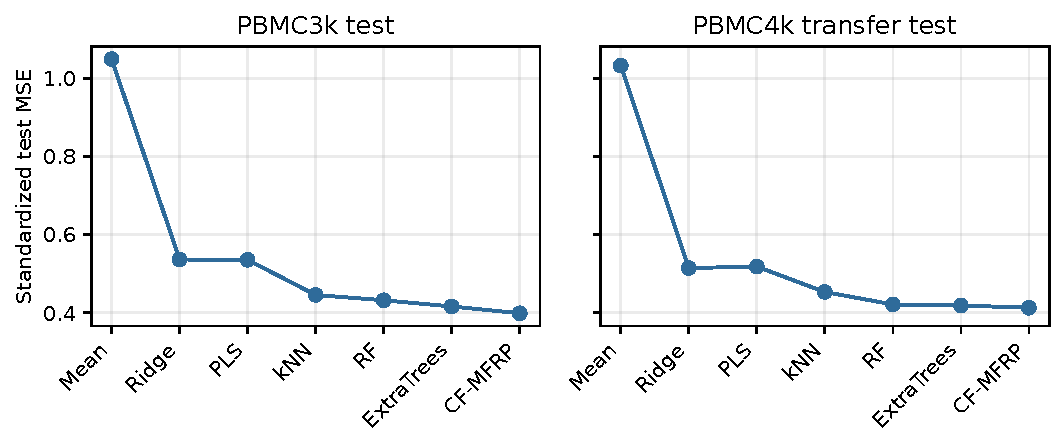
\includegraphics[width=0.82\textwidth]{code/manuscript_assets/figures/baseline_comparison.pdf}
\caption{Leakage-safe test MSE for every selected baseline and \method.  All
hyperparameters were selected on PBMC3k development cells; PBMC4k uses their
frozen values.  The former graph method is absent because the audit rejected it.}
\label{fig:baselines}
\end{figure}

\begin{table}[t]
\caption{Test metrics after family-wise development selection on PBMC3k.  Lower
is better.  PBMC4k is a frozen-parameter transfer, not a donor-population test.}
\label{tab:baselines}
\centering
\begin{tabular}{lrrrr}
\toprule
Method & PBMC3k MSE & PBMC3k MAE & PBMC4k MSE & PBMC4k MAE\\
\midrule
Mean & 1.0489 & 0.7097 & 1.0321 & 0.6983\\
Ridge & 0.5362 & 0.4584 & 0.5143 & 0.4558\\
PLS & 0.5353 & 0.4618 & 0.5180 & 0.4591\\
$k$NN & 0.4455 & 0.3410 & 0.4531 & 0.3628\\
Random forest & 0.4319 & 0.3648 & 0.4212 & 0.3728\\
ExtraTrees & 0.4160 & 0.3620 & 0.4186 & 0.3717\\
CF-MFRP & 0.3986 & 0.3350 & 0.4128 & 0.3521\\
\bottomrule
\end{tabular}

\end{table}

Figure~\ref{fig:baselines} and Table~\ref{tab:baselines} show the required
strong-baseline correction.  ExtraTrees is the best uncorrected method on both
tests.  \method\ lowers PBMC3k MSE by \PrimaryRelativeGain\ and PBMC4k MSE by
\ExternalRelativeGain.  These are two dataset-specific observations.  They do
not establish universal superiority over tree ensembles or specialist
single-cell methods.

\begin{figure}[t]
\centering
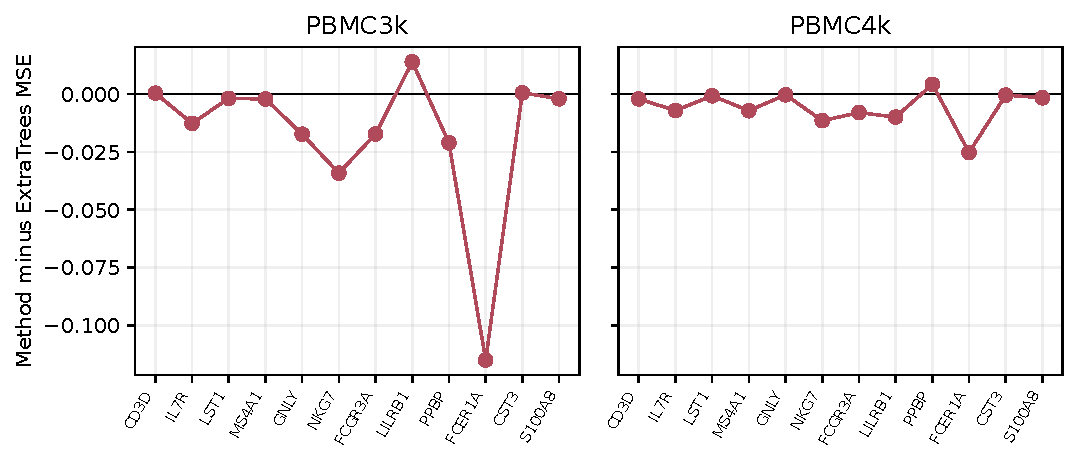
\includegraphics[width=0.88\textwidth]{code/manuscript_assets/figures/gene_differences.pdf}
\caption{Gene-resolved change relative to ExtraTrees.  Values below zero favor
the correction.  Aggregate improvement coexists with target-specific losses.}
\label{fig:genes}
\end{figure}

\begin{table}[t]
\caption{Gene-level MSE.  ET denotes ExtraTrees; CF denotes \method; $\Delta$
is corrected minus ExtraTrees MSE.}
\label{tab:genes}
\centering
\begin{tabular}{lrrrrrr}
\toprule
Gene & 3k ET & 3k CF & $\Delta$3k & 4k ET & 4k CF & $\Delta$4k\\
\midrule
CD3D & 0.4478 & 0.4482 & +0.0004 & 0.3544 & 0.3523 & -0.0021\\
IL7R & 0.6558 & 0.6431 & -0.0127 & 0.5576 & 0.5505 & -0.0071\\
LST1 & 0.1929 & 0.1910 & -0.0019 & 0.1911 & 0.1904 & -0.0007\\
MS4A1 & 0.3398 & 0.3377 & -0.0021 & 0.2223 & 0.2151 & -0.0072\\
GNLY & 0.4941 & 0.4768 & -0.0173 & 0.5137 & 0.5134 & -0.0003\\
NKG7 & 0.3336 & 0.2994 & -0.0342 & 0.2431 & 0.2316 & -0.0115\\
FCGR3A & 0.3296 & 0.3124 & -0.0173 & 0.3285 & 0.3205 & -0.0080\\
LILRB1 & 0.7319 & 0.7459 & +0.0139 & 0.8241 & 0.8142 & -0.0100\\
PPBP & 0.4056 & 0.3845 & -0.0211 & 1.1220 & 1.1262 & +0.0042\\
FCER1A & 0.7376 & 0.6226 & -0.1151 & 0.3124 & 0.2871 & -0.0253\\
CST3 & 0.1750 & 0.1756 & +0.0006 & 0.1825 & 0.1821 & -0.0005\\
S100A8 & 0.1487 & 0.1467 & -0.0020 & 0.1714 & 0.1698 & -0.0016\\
\bottomrule
\end{tabular}

\end{table}

The correction wins for 9 of 12 targets on PBMC3k and 11 of 12 on PBMC4k
(Fig.~\ref{fig:genes}, Table~\ref{tab:genes}).  The losing genes are retained.
No marker is converted into a cell-type or functional conclusion.
Figure~\ref{fig:path} isolates development-only selection, and
Fig.~\ref{fig:splits} retains the sign and magnitude of all five split audits.

\begin{figure}[t]
\centering
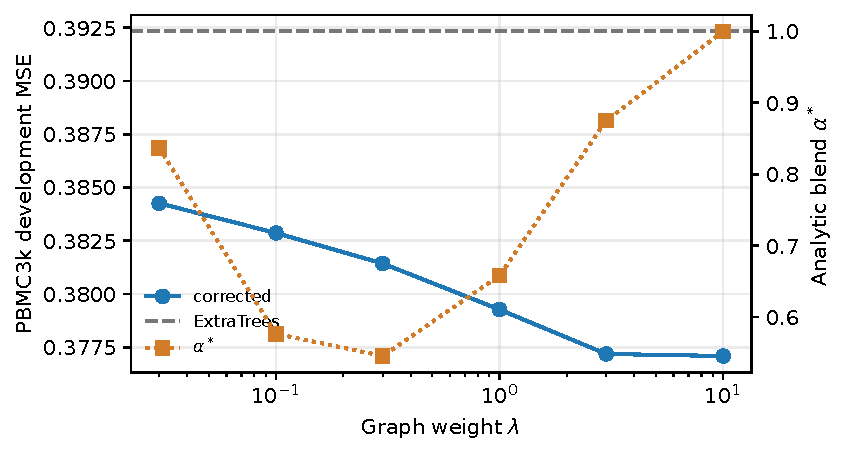
\includegraphics[width=\columnwidth]{code/manuscript_assets/figures/regularization_path.pdf}
\caption{PBMC3k development-only selection.  The blend is computed analytically
for each graph weight; test errors are not present in this artifact.}
\label{fig:path}
\end{figure}

\begin{figure}[t]
\centering
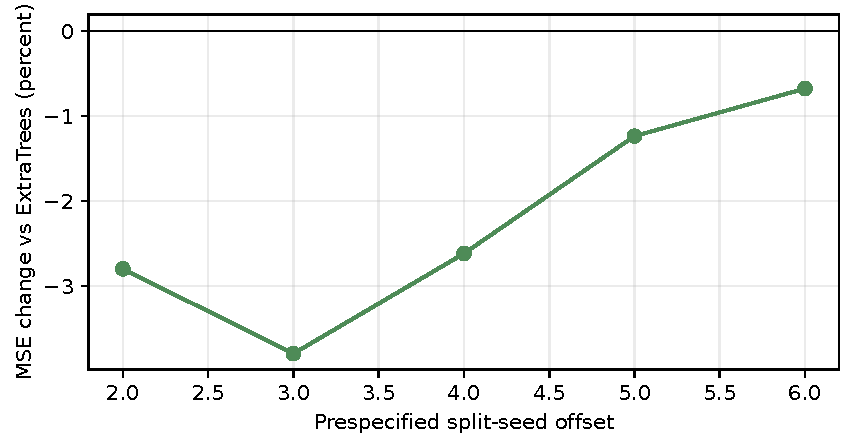
\includegraphics[width=\columnwidth]{code/manuscript_assets/figures/split_stability.pdf}
\caption{Five frozen-parameter PBMC3k split audits.  Negative values favor
\method.  Overlapping cells make these sensitivity checks, not independent
replicates or confidence intervals.}
\label{fig:splits}
\end{figure}

All five repeated splits favor the correction (\RepeatWins{} of 5), with relative
MSE changes ranging from approximately $-0.7\%$ to $-3.8\%$.  This reduces
concern that the sign is unique to one cell permutation, but it does not add
donors.

\begin{table}[t]
\caption{Sparse-operator and PCG certificates for the two final recovery runs.}
\label{tab:numerics}
\centering
\begin{tabular}{lrrrrr}
\toprule
Source & $n$ & nnz$(P)$ & CSR/dense & Iterations & Max residual\\
\midrule
pbmc3k & 2700 & 40500 & 0.0115 & 49 & 9.63e-10\\
pbmc4k & 4340 & 65100 & 0.0071 & 50 & 9.60e-10\\
\bottomrule
\end{tabular}

\end{table}

The PBMC3k graph stores \PrimaryStorage\ of the value-plus-index scalar count of
a dense matrix; PBMC4k stores \ExternalStorage.  Maximum relative residuals are
\PrimaryResidual\ and \ExternalResidual.  Explicit dense controls at
$n\in\{64,128,256\}$ agree with the matrix-free solution to at worst
$1.90\times10^{-10}$.  This validates implementation of the declared equation,
not the graph model.  Table~\ref{tab:numerics} gives the storage and residual
certificates supporting that implementation check.

\begin{figure}[t]
\centering
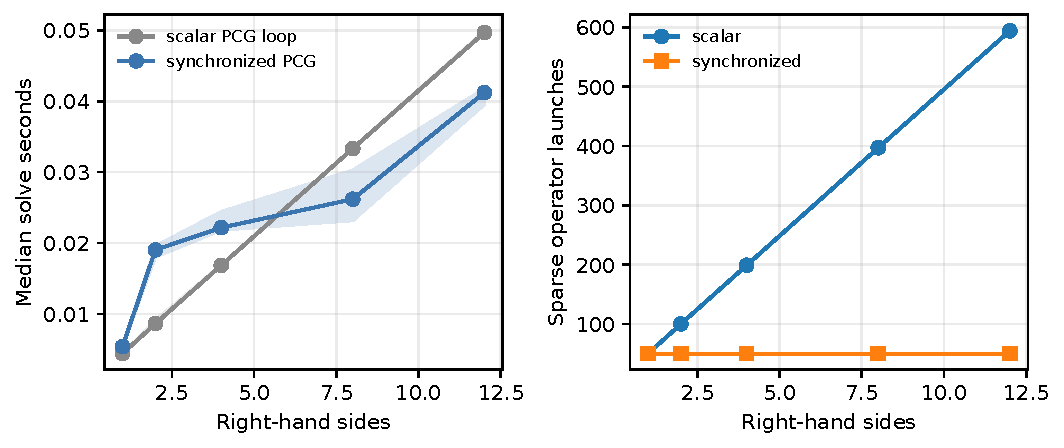
\includegraphics[width=0.86\textwidth]{code/manuscript_assets/figures/solver_scaling.pdf}
\caption{Bounded PBMC3k solve audit: medians and interquartile ranges over seven
alternating-order repetitions (left), and sparse operator launches (right).
Synchronized PCG loses for one to four right-hand sides and wins for eight and
twelve on this environment.  The twelve-column solutions agree with scalar PCG
to \BatchAgreement.}
\label{fig:solver}
\end{figure}

Figure~\ref{fig:solver} is deliberately not summarized as a universal speedup.
At twelve right-hand sides the measured scalar-to-synchronized ratio is
\BatchSpeedRatio, but at one, two, and four right-hand sides the synchronized
Python/SciPy path is slower.  Threading, cache, sparse layout, and hardware can
move the crossover.  The robust computational claims are the storage bound,
operator-launch count, residual, and scalar equivalence.

\section{Reproducibility and limitations}

The public package contains both original CC BY 4.0 archives, their SHA-256
digests, source attribution, deterministic seeds, selected Ensembl IDs, all
tuning rows without test metrics, fold-level zero-overlap audits, locked JSON,
generated TeX tables, figure code, and tests.  The principal commands are
\begin{verbatim}
python -m pip install --only-binary=:all: \
  -r code/requirements-lock.txt
python -m pip install --no-deps ./code
mfcell-reproduce --verify
python code/scripts/validate_release.py
\end{verbatim}
Clean replay within the registered reference environment compares discrete
protocol fields and digests exactly and
floating evidence within relative tolerance $0.5\%$ and absolute tolerance
$5\times10^{-5}$; environment and runtime fields are excluded.  It recomputes
archive statistics, feature selection, model selection, both final tests,
repeated splits, dense controls, gene-level rank correlations, and
scalar--batched agreement.

The limitations are material.  First, the test outcomes were observed during
this repair, so this is not prospective confirmation.  Second, two donors are
not a donor population; PBMC4k and PBMC3k also differ in reference build and
Cell Ranger version.  Third, a random cell split is easier than a donor-held-out
clinical task.  Fourth, target-excluded library normalization defines a clear
masked-gene estimand but is not asserted to be optimal single-cell
normalization.  Fifth, ExtraTrees and the listed simple baselines are strong for
this sample size, yet the experiment does not exhaust all probabilistic or deep
single-cell models.  Sixth, standardized MSE can reward shrinkage and does not
measure covariance preservation or latent molecule truth.  Seventh, the graph
uses test covariates and is transductive.  Finally, synchronized PCG changes
launch granularity, not the mathematical estimator or worst-case arithmetic
order.

The next defensible study would freeze this protocol before acquiring multiple
donors, evaluate donor-held-out panels and covariance distortion, and compare
against specialist count models under matched tuning budgets.  Until then, the
evidence supports a reproducible two-source numerical finding and the stated
finite-dimensional bounds---nothing broader.

\appendix

\section{Target-label noninterference}

\begin{proposition}[Sealed test targets]
After PBMC3k development selection is frozen, each test prediction is a
deterministic function of public constants, all non-target covariates, training
targets, fold assignments, and the graph; it is independent of test-target
entries as program inputs.
\end{proposition}
\begin{proof}
Equation~\eqref{eq:normalization} removes every target count from the exposure,
so input normalization is a function of non-target counts alone.  Input-gene
selection, standardization, PCA, and graph construction consume only those
inputs and training indices.  The full base learner consumes training targets;
each out-of-fold seed additionally excludes its own fold targets from its fitted
model.  Equation~\eqref{eq:system} has right side $MR$, which is zero outside
training cells.  The frozen $\lambda$ and $\alpha$ are constants on the final
test runs.  Composition of these maps therefore contains no test-target
argument.  Test targets enter only the subsequent metric computation.
\end{proof}

This is an information-flow proof for the implementation contract.  It does
not make test cells statistically independent, because their graph covariates
and biological source are shared.

\section{Conditioning and classical PCG bound}

Because $0\preceq M\preceq I$ and
$\norm{D}_2\le1+\norm{P}_2$,
\begin{equation}
 \lambda_{\max}(A_\lambda)
 \le1+\mu+\lambda(1+\norm{P}_2)^2,
\end{equation}
whereas $\lambda_{\min}(A_\lambda)\ge\mu$.  Therefore
\begin{equation}
 \kappa_2(A_\lambda)\le
 \frac{1+\mu+\lambda(1+\norm{P}_2)^2}{\mu}.
\end{equation}
For unpreconditioned CG, the standard energy-norm estimate is
\begin{equation}
 \frac{\norm{e_m}_{A_\lambda}}{\norm{e_0}_{A_\lambda}}
 \le2\left(\frac{\sqrt\kappa-1}{\sqrt\kappa+1}\right)^m.
\end{equation}
The implementation uses a Jacobi preconditioner and reports actual residuals;
it does not substitute this conservative bound for a measured stopping test
\cite{hestenes1952methods,saad2003iterative,benzi2002preconditioning}.

\section{Software and environment boundary}

NumPy, SciPy, scikit-learn, and Matplotlib provide the array, sparse solve,
baseline, and plotting layers~\cite{harris2020array,virtanen2020scipy,
pedregosa2011scikit}.  Random seeds fix splits, forests, and folds.  Scientific
floats are compared within declared tolerances across a fresh replay.  Wall
times are excluded because they depend on the current Python, library, CPU,
thread, and power state.  The release records those fields rather than hiding
them.

\bibliographystyle{plainnat}
\bibliography{code/manuscript_assets/references}

\end{document}
